\documentclass[tikz, border=3mm]{standalone}
\usepackage{tikz}
\usetikzlibrary{
    arrows.meta,         % For arrow tips
    decorations.markings,% For placing arrows along paths
    positioning          % For label positioning
}

\begin{document}
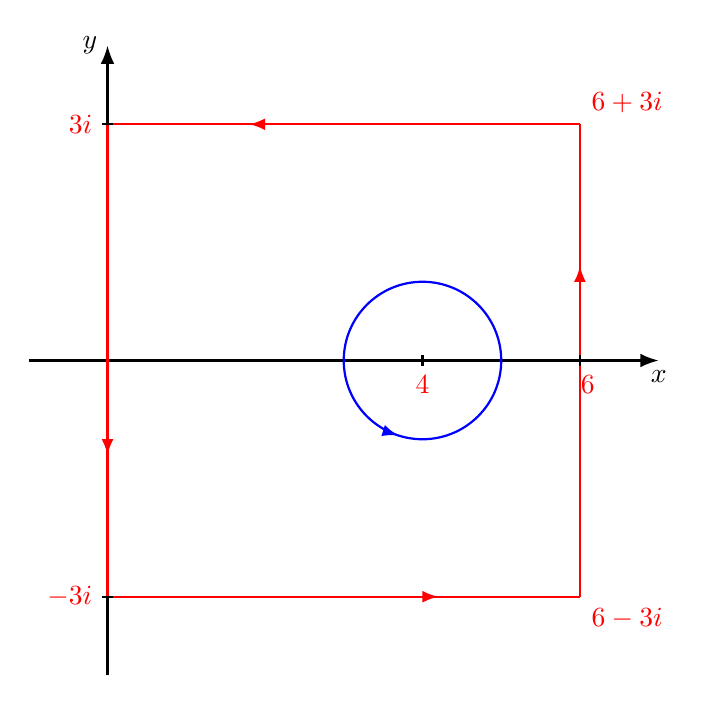
\begin{tikzpicture}[
    >=Latex, % Set default arrow tip style
    axis/.style={->, thick}, % Style for axes
    contour/.style={thick},    % Base style for contours
    % Style for placing a CCW arrow (>) on a path
     midarrow/.style={
        decoration={markings, mark=at position 0.7 with {\arrow{Latex[length=2mm]}}},
        postaction={decorate}
    },
    midarrowL/.style={
        decoration={markings, mark=at position 0.2 with {\arrowreversed{Latex}}},
        postaction={decorate}
    },
    labelstyle/.style={red}, % Style for red labels
    tick/.style={thick} % Style for tick marks
]

    % Axes (adjust limits as needed)
    \draw[axis] (-1, 0) -- (7, 0) node[below] {$x$};
    \draw[axis] (0, -4) -- (0, 4) node[left] {$y$};

    % Define Rectangle Corners
    \coordinate (TL) at (0, 3);  % Top Left
    \coordinate (TR) at (6, 3);  % Top Right
    \coordinate (BR) at (6, -3); % Bottom Right
    \coordinate (BL) at (0, -3); % Bottom Left

    % Define Circle Center and Radius
    \coordinate (CircCenter) at (4, 0);
    \def\radius{1.0} % Adjust radius as needed

    % Draw Rectangular Contour (Red, CCW)
    \draw[contour, red, midarrow] (BL) -- (BR); % Bottom edge, arrow right
    \draw[contour, red, midarrow] (BR) -- (TR); % Right edge, arrow up
    \draw[contour, red, midarrow] (TR) -- (TL); % Top edge, arrow left
    \draw[contour, red, midarrow] (TL) -- (BL); % Left edge, arrow down

    % Draw Inner Circle (Blue, CW)
    % Draw the circle path first
    \draw[contour, blue] (CircCenter) circle (\radius);
    % Add the arrow decoration separately using postaction on the path
    \path[contour, blue, midarrow] (CircCenter) circle (\radius); % Arrow near top (pos 0.25)

    % Ticks on axes
    \draw[tick] (4, -2pt) -- (4, 2pt);   % Tick at x=4 (circle center)
    \draw[tick] (6, -2pt) -- (6, 2pt);   % Tick at x=6 (rectangle edge)
    \draw[tick] (-2pt, 3) -- (2pt, 3);   % Tick at y=3 (rectangle edge)
    \draw[tick] (-2pt, -3) -- (2pt, -3); % Tick at y=-3 (rectangle edge)

    % Labels
    \node[labelstyle, left=2pt] at (TL) {$3i$};
    \node[labelstyle, above right=1pt] at (TR) {$6+3i$};
    \node[labelstyle, below right=1pt] at (BR) {$6-3i$};
    \node[labelstyle, left=2pt] at (BL) {$-3i$};
    \node[labelstyle, below=2pt] at (CircCenter) {$4$};
    \node[labelstyle, below=2pt] at (6.1, 0) {$6$};

\end{tikzpicture}
\end{document}